\documentclass[conference]{IEEEtran}
\usepackage{amsmath,amssymb,graphicx,booktabs,tabularx,array,cite}
\usepackage[hidelinks]{hyperref}
\usepackage{microtype}
\newcolumntype{Y}{>{\raggedright\arraybackslash}X}
\graphicspath{{figures/}}
\begin{document}
\title{Resilient Task Offloading under Network Stress and Energy Variability in IIoT}
\author{\IEEEauthorblockN{Sanya Chavan}\IEEEauthorblockA{IT Department / K J Somaiya School of Engineering\\Maharashtra, India}}
\maketitle
\begin{abstract}
The energy benefit of industrial edge offloading depends on communication service, task deadlines, and battery supply. We study these dependencies using frozen QECO checkpoints, traffic-derived effective-capacity scenarios, explicit power--time accounting, and a battery-aware extension driven by the UCLM outdoor harvesting trace. On 1,000 paired workload episodes, a decision-time selector reduces user-equipment energy by 7.02\% and deadline-violation counts by 45.39\% at Medium stress relative to original QECO. Always-Local, Fixed-Edge-0, and a greedy energy/deadline rule expose the energy--service tradeoff; low expenditure alone does not establish better service. An additional five-workload-seed experiment evaluates the frozen-policy comparison with seed-level uncertainty. Five independently trained EH models are evaluated with harvesting enabled and disabled on the same 110-second test window; nested episodes are averaged within each seed before inference. Harvesting produces a small positive battery-reserve difference, while every two-sided exact seed-level test of the reported EH energy and reserve effects has $p=0.0625$. Combining the selector with EH-QECO improves deadline service while increasing expenditure relative to the largely local EH policy. Analytical stress-exponent sensitivity and deterministic battery-demand replay quantify parameter dependence. These results support an auditable simulation framework and conditional offloading decisions, rather than hardware validation, a calibrated wireless degradation law, or a large EH performance gain.
\end{abstract}
\begin{IEEEkeywords}
Industrial Internet of Things, mobile edge computing, task offloading, energy harvesting, deep reinforcement learning, reproducibility.
\end{IEEEkeywords}

\section{Introduction}
Industrial endpoints must balance computation, communication, and timely service. Edge offloading can replace local CPU work with radio transmission and remote waiting; whether that replacement saves device energy depends on the operating condition. Surveys describe multiple task-offloading architectures and objectives \cite{Islam2021_supp11,Wang2020_supp14,Yang2023_supp18}. Industrial edge deployments and monitoring systems provide application context \cite{Donovan2022_supp8,Singh2024_supp3,Mirani2024_supp7}; they do not validate the offloading policy studied here.

QECO combines dueling double deep Q-learning with recurrent state for QoE-oriented computation offloading \cite{QECO,QECOCode}. We freeze its supplied checkpoints to study sensitivity to communication service, then apply a decision-time selector without learning. Separately, EH-QECO augments the observation with battery reserve and harvesting availability. The resulting experiments address three questions: how traffic-derived service scenarios affect a fixed policy; whether action correction improves its energy--deadline tradeoff; and how measured renewable input affects a retrained policy's battery ledger.

The contributions are a controlled stress replay with three quantitative comparator rules; independent workload-seed validation of the frozen policy and training-seed analysis of the EH branch; corrected matched-task forecasts using each policy's executed trajectory; a combined selector/EH experiment; and a reproducibility package that generates the numerical tables from saved records. All hardware powers, stress weights, and conversion efficiencies are explicit assumptions. No claim is made that the selector outperforms every baseline on every objective.

\subsection{Related Work and Scope}
Industrial latency-critical offloading \cite{Mali2024_s3}, joint offloading/resource allocation \cite{Jiang2023_s30}, adaptive matching \cite{Chi2024_s26}, partial offloading in multi-RAT networks \cite{Qin2021_s31}, and digital-twin-aided edge selection \cite{DoDuy2022_s17} establish relevant decision contexts. EH offloading has been studied through dynamic optimization and learning \cite{Mao2016_s2,Min2017_s18,Mei2023_s23}. These works motivate energy availability as a system state; their numerical gains are not transferred to this study.

\begin{table}[t]
\centering\small
\caption{Scope of the present comparison}
\label{tab:scope}
\begin{tabularx}{\columnwidth}{@{}lY@{}}\toprule
Evidence & Role and boundary\\\midrule
QECO \cite{QECO} & Supplied checkpoints; fixed-policy service sensitivity.\\
EH offloading \cite{Mao2016_s2,Min2017_s18,Mei2023_s23} & Motivation for battery and renewable-input states.\\
Industrial monitoring \cite{Singh2024_supp3,Mirani2024_supp7} & Application context; separate from policy validation.\\
Traffic \cite{Traffic} and UCLM \cite{UCLM,UCLMData} & Empirical inputs to simulated execution.\\\bottomrule
\end{tabularx}
\end{table}
The literature component is a focused contextual synthesis, not an exhaustive systematic review or an independent deployment census. The inherited 31-study coding matrix is retained in the supplementary archive for traceability, but broad corpus percentages are not used as experimental evidence. This reduces space and avoids implying that every inherited bibliographic or classification entry has been independently revalidated.

\section{System Model and Method}
\label{sec:method}
\subsection{Frozen QECO and Workload}
There are 20 user-equipment devices (UEs), two edges, and three actions: local, edge 0, and edge 1. Each episode has 110 slots of $\Delta t=0.1$\,s. Task sizes are in $[1,7]$ simulator data units, computation densities in $\{0.197,0.297,0.397\}$, and arrivals occur with probability 0.3 per UE per active slot. The last ten slots have no new arrivals; every task has a ten-slot (1\,s) deadline. UE and edge computation capacities are 2.6 and 42 simulator work units per second. These are abstract simulator units, not claimed measurements of bits, cycles, or a named industrial device.

The frozen branch uses the repository's 20 per-UE PerformanceMode/800 checkpoints with greedy evaluation and no updates. The original six-feature observation includes the task, queue, energy-preference, and edge-backlog information supplied by the implementation. Its static energy-preference values are not physical SOC. Existing observation bookkeeping behavior is preserved for this fixed-checkpoint audit, so conclusions describe the audited implementation rather than a corrected, retrained QECO baseline. The first replay uses the 1,000 saved workloads of the frozen artifact. The additional validation uses five independent workload generators with seeds 1101, 2202, 3303, 4404, and 5505, ten episodes each, and the same checkpoints. These are workload seeds, not independent QECO training seeds.

\subsection{Energy Accounting and Deadline Metrics}
Configured UE CPU, radio, and idle powers are 2.0, 2.3, and 0.1\,W; edge CPU power is 5.0\,W. The evaluation ledger records serviced work, including work spent on tasks that later fail. For each UE and slot, CPU and radio activity fractions $\ell$ and $x$ are obtained from actually processed volumes. Post-transmission waiting is charged as a union of waiting intervals, excluding overlapping CPU/radio activity. Thus
\begin{equation}
E_{\rm UE}=\Delta t\sum_{u,t}(P_l\ell_{u,t}+P_xx_{u,t}+P_iw_{u,t}),
\label{eq:energy}
\end{equation}
where $w$ is the non-overlapping task-wait fraction. System energy adds share-allocated edge computation. Background idle outside task-related waiting is excluded from this ledger. Powers are uncalibrated scenario assumptions.

The violation rate is failed/deadline-expired tasks divided by arrivals. Terminal time includes both completion and expiry; completion time is used only for successfully completed tasks. Lower expenditure can result from incomplete work, so energy is always interpreted alongside violations and offloading fraction.

\subsection{Traffic-Derived Communication Stress}
The smart-factory traffic dataset concerns malware communication \cite{Traffic}, not measured wireless capacity. Frozen development inputs contain 195,806 windows (191,008 BENIGN and 4,798 ABNORMAL); only sources a\_day1 and s\_day1 contain both labels and enter the source-matched severity calculation. All 4,798 ABNORMAL windows and 13,186 BENIGN windows in those sources define the reported profiles. ABNORMAL is not relabeled as a physical congestion measurement. Classifier predictions and held-out classifier data do not enter the offloading simulation.

Two author-defined weight sets serve different purposes. The severity score weights source-normalized benign percentiles of packet rate, new flows, unique sources, unique destinations, short-flow churn, and persistent-flow occupancy. The weights are 0.35, 0.20, 0.10, 0.10, 0.15, and 0.10. Within-source ABNORMAL terciles determine Low, Medium, and High labels. Separately, the offered-load multiplier is the weighted geometric mean of packet-rate, new-flow, source-count, and destination-count ratios to source-specific benign medians, clipped below at one, with weights 0.70, 0.15, 0.075, and 0.075. Source-balanced medians and a monotonic envelope produce $M$.
\begin{equation}
C_{\rm eff}=14\max(M^{-\alpha},0.25),\qquad \alpha=1/2.
\label{eq:capacity}
\end{equation}
The weights prioritize packet activity and flow-state pressure as an engineering choice. They are not estimated from a queueing law, calibrated to RF measurements, or established by literature. The square root compresses the multiplier as an author-defined sensitivity proxy; it is not an M/M/1 derivation. Exponent sensitivity is quantified in Section~\ref{sec:sensitivity}; weight sensitivity has not been validated. No fading, interference, loss, retransmission, or jitter process is invented.
\begin{table}[t]
\centering\footnotesize
\caption{Traffic-derived profile and simulated service.}
\label{tab:stress}
\begin{tabular}{@{}lrrr@{}}\toprule
Label & Windows & $M$ & $C_{\rm eff}$\\\midrule
Normal & 13186 & 1.0000 & 14.0000 \\
Low & 1600 & 1.0000 & 14.0000 \\
Medium & 1598 & 2.7207 & 8.4877 \\
High & 1600 & 4.8964 & 6.3269 \\
\bottomrule\end{tabular}
\end{table}

Normal and Low map to identical capacity 14.0; they are the same simulated service condition. Quantitative comparisons use Normal, Medium, and High only.

\subsection{Matched-Task Counterfactual and Energy Boundary}
\label{sec:matched}
Counterfactual analysis uses each policy's saved executed actions and its own queue trajectory, rather than proposed original actions inside the selector trajectory. For the first 100 paired saved episodes per condition, deterministic action replay must reproduce the saved delays and transmitted volumes. At each actual offload decision, the local FIFO forecast includes known backlog but excludes future arrivals. An infeasible local forecast is censored after the deadline and is not reported as an actual completion.

For a task of size $s$ and density $\rho$, the equal-work local service requirement and full-transmission requirement are
\begin{equation}
E_l^{\rm full}=P_l s\rho/C_l,\qquad E_x^{\rm full}=P_x s/C_{\rm eff}.
\label{eq:matched}
\end{equation}
The offload full-work attribution adds 0.1\,W times the task's observed post-transmission wait. This is a per-task attribution, distinct from the union-based episode ledger. The table reports these requirements, actual expended TX energy, forecast local feasibility, and observed offload success on the same offloaded-task cohort. Completion times are compared only on the intersection of locally predicted-feasible and actually successful offloaded tasks. Changing a whole policy would alter future queues; this analysis is a conditional forecast, not an executed Always-Local rerun.

Transmission-only break-even capacity is
\begin{equation}
C_x^*(\rho)=\frac{P_xC_l}{P_l\rho}.
\label{eq:crossover}
\end{equation}
For the three densities it is 15.18, 10.07, and 7.53 units/s. All exceed High's 6.3269. This is an equal-full-work boundary under the configured powers; early expiry can reduce observed expenditure, and task-wait energy raises the true full-offload requirement. An aggregate policy crossover is not located by this equation.

\subsection{Selector and Comparator Rules}
At each arrival, the selector forecasts local and both edge alternatives from the common pre-step state. Known FIFO backlog is simulated without future arrivals; edge service assumes the current active-user share. Among predicted deadline-feasible actions, it minimizes predicted UE energy. It retains QECO on a minimum-energy tie, otherwise uses deterministic action-order tie-breaking. If no action is predicted feasible, it retains QECO. No future arrival or realized outcome is available to the decision.

Always-Local chooses local on every arrival; Fixed-Edge-0 always chooses edge 0. The additional Greedy rule uses the same forecasting machinery but never consults D3QN: it chooses a feasible minimum-energy action, breaks ties in local/edge-0/edge-1 order, and chooses the smallest predicted terminal delay if none is feasible. This is an author-defined rule rather than a reimplementation of a published competing DRL algorithm. Its large similarity to the selector makes it an informative test of whether the learned proposal itself adds value.

\section{Energy-Harvesting Extension}
\label{sec:ehmethod}
\subsection{Trace, Partitions, and Actual Coverage}
UCLM provides an outdoor IoT harvesting trace \cite{UCLM,UCLMData}. Raw timestamps, currents, and voltage are preserved. Table~\ref{tab:split} gives the exact row-defined chronological partitions. The 93,438 observations span 66 calendar dates, with an elapsed duration of 64\,days 23\,h 35\,min 56\,s. Nominal cadence is one minute; observed intervals comprise 32 at 59\,s, 85,213 at 60\,s, 8,191 at 61\,s, and one 237\,s gap.
\begin{table*}[t]
\centering\footnotesize
\caption{Exact UCLM row partitions. Elapsed durations are end timestamp minus start timestamp, not counts of full days.}
\label{tab:split}
\begin{tabular}{@{}lrllll@{}}\toprule
Partition & Rows & First timestamp & Last timestamp & Elapsed & Purpose\\\midrule
Train & 56726 & 2018-07-31 13:07:15 & 2018-09-08 23:59:56 & 39d 10h 52m 41s & Training allocation; initial 19 rows consumed \\
Val & 18686 & 2018-09-09 00:00:56 & 2018-09-21 23:59:58 & 12d 23h 59m 2s & Reserved; unused in model selection \\
Test & 18026 & 2018-09-22 00:00:58 & 2018-10-04 12:43:11 & 12d 12h 42m 13s & Evaluation allocation; brief selected window \\
\bottomrule\end{tabular}
\end{table*}

There are no rows outside the three partitions. However, assigning a row to a partition is not evidence that it was consumed by a rollout. Each saved model trained for 100 episodes, 1,100\,s on the nominal time grid, using only the initial approximately 19 training rows. The validation partition was reserved but unused: no validation-based hyperparameter search or checkpoint selection is claimed. Core testing uses ten episodes per model, 110\,s, starting at test row 540 (raw timestamp 22 September 2018, 09:01:29), approximately two source records. It does not cover every test day. The main test window is a daytime scenario, not representative diurnal sampling.

The inherited simulation holds each record for 600 slots (60 nominal seconds); it does not replay the irregular timestamp intervals exactly. This nominal-grid approximation is retained to reproduce the reported experiments, with timestamps used for partition identification. A claim of exact wall-clock trace replay would therefore be inappropriate.

\subsection{Battery Ledger and Observation}
Positive battery current is treated as charging in the trace reconstruction; the external-source proxy is $I_h=\max(I_{\rm node}+I_{\rm battery},0)$. This assumes currents meet at a common bus and neglects converter losses beyond the stated efficiency. It is a modelling reconstruction, not measured PV maximum-power-point output. PV short-circuit current is not converted to harvested power.

Stored charge $q$ in mAh is updated by
\begin{equation}
q_{t+1}=\left[\min(Q,q_t+\eta_c I_h\Delta t/3600)-\frac{1000P_b\Delta t}{3600V_t\eta_d}\right]_+,
\label{eq:battery}
\end{equation}
where $Q=2,000$\,mAh, initial SOC $q_0/Q=0.5$, and $\eta_c=\eta_d=0.95$. Efficiencies and initial SOC are assumptions. $V_t$ is the trace battery voltage with a 3.3\,V lower clamp, not a fixed 3.7\,V discharge voltage. The battery demand $P_b=P_l\ell+P_xx+P_i[1-\max(\ell,x)]_+$ includes background idle and concurrent CPU/radio demand. It therefore differs from the task-related energy ledger in Eq.~\eqref{eq:energy}; SOC cannot be derived by dividing the table's UE energy by nominal voltage.

Battery SOC and the trace pointer persist across the ten episodes; task queues reset. The eight-feature observation appends current SOC and $\min(I_h/500,1)$ to the original six features on active arrivals. No future harvesting values are supplied. EH training uses a shared D3QN network, one-step recurrent input with zero supplied recurrent histories, rather than the original 20-policy ten-step history configuration. Hence it has an LSTM layer but the experiment does not validate learned temporal harvesting prediction.

\subsection{Training and EH-Disabled Definition}
The five independent training seeds are 101, 202, 303, 404, and 505. Checkpoint hashes match the recorded metadata. Training uses Normal capacity, generated workloads, learning rate 0.002, discount 0.9, replay size 2,000, batch size 32, target replacement every 200 updates, and epsilon increasing by 0.002 to 0.98. The saved update counts are 10,990, 10,988, 10,991, 10,988, and 10,990 (54,947 total). The reward is
\begin{equation}
r=-2(1-\mathrm{SOC})-20U-0.15b-0.01a,
\label{eq:reward}
\end{equation}
where $U$ is cumulative unmet charge, $b$ is the maximum local/transmission backlog in slots, and $a\in\{0,1,2\}$. This is an author-defined reward and changes the original QECO objective; it does not explicitly penalize realized deadline failure.

EH-disabled is an \emph{evaluation ablation of the same EH-trained checkpoint}, not a separately retrained non-EH agent. It retains all eight features, the same seed/model, the same saved workloads 0000--0009, the same initial 50\% SOC, efficiencies, persistent battery, stress, and trace voltage. Harvest input and its observation feature are set to zero. SOC evolves under the no-harvest ledger. Each enabled/disabled condition starts from a new battery/trace instance, and evaluation is greedy. The comparison jointly changes energy input and observed current availability; it does not isolate the architectural benefit of observing SOC.

\subsection{Energy-Causality Boundary}
The inherited environment checks the charge needed for the proposed action and records insufficient-supply events. However, its fallback assigns local action and still calls the base service engine; it does not stall all ongoing CPU/radio service when charge is exhausted. Clipping charge at zero consequently enforces a bounded ledger, not strict execution-level energy causality. All core short rollouts remain above depletion with zero recorded insufficient-charge events, so this defect is inactive there. Post-depletion task-success and energy-failure counts from the old multi-hour runs are excluded from the conclusions. Hardware brownout prevention and causal battery-empty operation have not been established.

\section{Experimental Design and Statistical Analysis}
The 1,000-episode comparison is conditional on fixed checkpoints and saved workload sequence. Means, episode SDs, and Student-$t$ 95\% mean intervals are reported; paired differences use aligned episode indices. This estimates workload uncertainty under those checkpoints, not training uncertainty. The separate five-seed workload experiment averages ten episode metrics within each workload seed before inference.

For EH, each independent training seed contributes one mean over its ten nested episodes. No analysis treats five seeds times ten episodes as 50 independent trained models. Reported SD is the sample SD of five seed means; the mean interval is $\bar x\pm t_{0.975,4}s/\sqrt5$. Paired differences are computed seed-by-seed. Two-sided exact sign-flip tests enumerate all $2^5$ sign assignments and use absolute mean difference. Parametric paired-$t$ intervals describe uncertainty under normal seed-effect assumptions; the exact test has coarse resolution and need not agree with those intervals. Exact tests are the inferential basis for EH claims; no reported EH benefit meets the 0.05 threshold. Tests are exploratory across multiple stresses and outcomes.

Energy is a per-episode 20-UE total unless explicitly marked per task. SOC is reported in percent; an SOC difference is in percentage points (pp). The average of ten cumulative episode-end readings is not terminal SOC or total harvested charge. Terminal metrics use episode 9 only, after the full 110\,s.

\section{Results}
\subsection{Frozen-Policy Stress Replay and Baselines}
\begin{table*}[t]
\centering\footnotesize
\caption{1,000 saved-workload episodes per policy and condition. UE energy is mean $\pm$ episode SD; intervals are conditional on the fixed checkpoints.}
\label{tab:main}
\begin{tabular}{@{}llrrrrrr@{}}\toprule
Stress & Policy & UE energy (J) & UE 95\% CI & System (J) & TX (J) & Violations (\%) & Offload (\%)\\\midrule
Normal & Original & 434.38 $\pm$ 16.30 & [433.36, 435.39] & 488.91 & 263.79 & 7.45 $\pm$ 1.63 & 63.97 \\
Normal & Selector & 397.62 $\pm$ 16.07 & [396.62, 398.61] & 455.80 & 246.73 & 6.81 $\pm$ 1.90 & 63.55 \\
Normal & Always-Local & 361.46 $\pm$ 6.64 & [361.05, 361.87] & 361.46 & 0.00 & 52.74 $\pm$ 2.86 & 0.00 \\
Normal & Fixed-Edge-0 & 357.49 $\pm$ 9.43 & [356.91, 358.08] & 401.28 & 354.99 & 56.12 $\pm$ 2.52 & 100.00 \\
Normal & Greedy-Rule & 397.20 $\pm$ 15.97 & [396.21, 398.20] & 455.59 & 243.85 & 6.99 $\pm$ 2.01 & 63.15 \\
Medium & Original & 562.17 $\pm$ 17.48 & [561.08, 563.25] & 593.87 & 351.39 & 23.72 $\pm$ 2.44 & 56.47 \\
Medium & Selector & 522.69 $\pm$ 18.97 & [521.51, 523.86] & 554.44 & 246.87 & 12.94 $\pm$ 2.19 & 38.10 \\
Medium & Always-Local & 361.46 $\pm$ 6.64 & [361.05, 361.87] & 361.46 & 0.00 & 52.74 $\pm$ 2.86 & 0.00 \\
Medium & Fixed-Edge-0 & 422.99 $\pm$ 7.25 & [422.54, 423.44] & 444.37 & 422.79 & 69.61 $\pm$ 2.47 & 100.00 \\
Medium & Greedy-Rule & 510.80 $\pm$ 17.59 & [509.71, 511.89] & 545.35 & 228.46 & 12.19 $\pm$ 1.97 & 35.71 \\
High & Original & 614.07 $\pm$ 16.90 & [613.02, 615.12] & 629.33 & 387.24 & 36.86 $\pm$ 2.30 & 53.65 \\
High & Selector & 567.09 $\pm$ 19.53 & [565.88, 568.30] & 577.11 & 241.91 & 24.95 $\pm$ 2.37 & 27.05 \\
High & Always-Local & 361.46 $\pm$ 6.64 & [361.05, 361.87] & 361.46 & 0.00 & 52.74 $\pm$ 2.86 & 0.00 \\
High & Fixed-Edge-0 & 443.77 $\pm$ 6.37 & [443.38, 444.17] & 454.28 & 443.71 & 81.44 $\pm$ 1.90 & 100.00 \\
High & Greedy-Rule & 507.29 $\pm$ 16.94 & [506.24, 508.34] & 524.33 & 163.85 & 24.08 $\pm$ 2.13 & 19.83 \\
\bottomrule\end{tabular}
\end{table*}

The selector's Medium UE-energy reduction relative to QECO is 7.02\%; violation counts fall 45.39\%. High reductions are 7.65\% and 32.26\%, respectively. These relative count reductions are distinct from percentage-point changes in failure rates. Paired intervals and additional workload-seed results are reported in Table~\ref{tab:mainstats}.
\begin{table*}[t]
\centering\footnotesize
\caption{Paired Selector minus Original. Five-workload-seed rows show mean difference $\pm$ seed SD (ten episodes per seed). Saved-replay tests use 10,000 random sign flips with a plus-one correction.}
\label{tab:mainstats}
\begin{tabular}{@{}lllrrr@{}}\toprule
Stress & Unit & Metric & Difference & 95\% CI & $p$\\\midrule
Normal & Saved 1,000 & UE (J) & -36.76 & [-37.02, -36.50] & 0.0001 \\
Normal & Saved 1,000 & Viol. (pp) & -0.64 & [-0.75, -0.53] & 0.0001 \\
Medium & Saved 1,000 & UE (J) & -39.48 & [-39.83, -39.13] & 0.0001 \\
Medium & Saved 1,000 & Viol. (pp) & -10.78 & [-10.89, -10.67] & 0.0001 \\
High & Saved 1,000 & UE (J) & -46.98 & [-47.43, -46.53] & 0.0001 \\
High & Saved 1,000 & Viol. (pp) & -11.91 & [-12.02, -11.80] & 0.0001 \\
Normal & 5 seeds & UE (J) & -37.10 $\pm$ 1.95 & [-39.52, -34.68] & 0.0625 \\
Normal & 5 seeds & Viol. (pp) & -0.45 $\pm$ 0.75 & [-1.39, 0.48] & 0.2500 \\
Medium & 5 seeds & UE (J) & -38.77 $\pm$ 1.83 & [-41.05, -36.49] & 0.0625 \\
Medium & 5 seeds & Viol. (pp) & -11.20 $\pm$ 0.72 & [-12.09, -10.30] & 0.0625 \\
High & 5 seeds & UE (J) & -45.55 $\pm$ 2.27 & [-48.37, -42.73] & 0.0625 \\
High & 5 seeds & Viol. (pp) & -12.00 $\pm$ 0.92 & [-13.14, -10.85] & 0.0625 \\
\bottomrule\end{tabular}

\par\smallskip\begin{minipage}{\textwidth}\footnotesize Seeds vary workloads; supplied QECO checkpoints stay fixed. The exact five-seed test has coarse resolution. All tests are exploratory and unadjusted; 1,000-episode intervals estimate conditional workload variability.\end{minipage}
\end{table*}

Always-Local uses less energy than the selector under some conditions but misses more deadlines. Fixed-Edge-0 incurs heavy radio expenditure and increasing violations as capacity falls. Greedy achieves a strong service--energy tradeoff; the selector cannot claim a general advantage over it. Baseline episode CIs reflect uncertainty over this particular replay workload distribution. Deterministic policy rules have no training seeds.

\begin{figure}[t]\centering
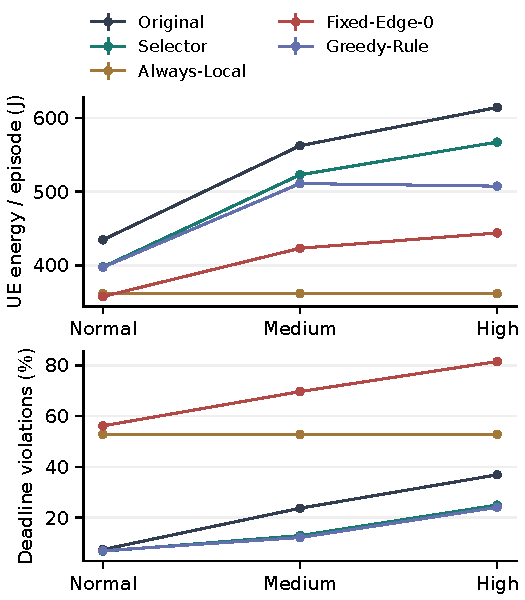
\includegraphics[width=\columnwidth]{comparison.pdf}
\caption{Paired saved-workload replay: UE energy and deadline violations are shown together. All three conditions have 1,000 episodes. Points use mean episode rates; error bars are 95\% mean intervals. Lower energy alone is insufficient to rank policies.}
\label{fig:comparison}\end{figure}

\subsection{Corrected Matched-Task Audit}
\begin{table*}[t]
\centering\footnotesize
\caption{Matched-task audit on 20 paired episodes per condition. Energy is per task; every deadline is 1.0\,s. Completion means use the same both-feasible task subset.}
\label{tab:counter}
\begin{tabular}{@{}llrrrrrrrr@{}}\toprule
Stress & Policy & Tasks & $E_l^{\rm full}$ & $E_x^{\rm full}+E_w^{\rm obs}$ & Actual TX & $T_l$ & $T_o$ & Local feas. & Offload succ.\\\midrule
Normal & Original & 7684 & 0.961 & 0.707 & 0.689 & 0.570 & 0.549 & 83.9 & 95.2 \\
Normal & Selector & 7593 & 1.049 & 0.672 & 0.649 & 0.591 & 0.610 & 84.2 & 90.6 \\
Medium & Original & 6807 & 0.955 & 1.141 & 1.034 & 0.558 & 0.698 & 77.7 & 67.6 \\
Medium & Selector & 4623 & 1.132 & 1.139 & 1.073 & 0.674 & 0.636 & 44.3 & 78.8 \\
High & Original & 6474 & 0.945 & 1.518 & 1.202 & 0.513 & 0.739 & 75.0 & 43.5 \\
High & Selector & 3234 & 1.223 & 1.779 & 1.484 & -- & -- & 0.0 & 38.9 \\
\bottomrule\end{tabular}

\par\smallskip\begin{minipage}{\textwidth}\footnotesize $E_l^{\rm full}$ is full local service energy in J. The offload column combines full-transmission requirement with observed per-task post-transmission waiting energy; it is not an observed successful full-offload requirement for expired tasks. Actual TX is spent energy, including expired transmissions. $T_l$ is a no-future-arrivals FIFO prediction and $T_o$ is observed successful completion (s), restricted to the intersection of local predicted feasibility and actual offload success. Feasibility/success columns (\%) use all offloaded tasks. A dash means an empty both-feasible subset, not zero completion time.\end{minipage}
\end{table*}

The local counterfactual and actual offload refer to the same offloaded tasks, but only the local outcome is a decision-time forecast. Completion means on the both-feasible cohort avoid treating expired tasks as completed. Full-work energy requirements can exceed actually expended TX energy because transmission may end at expiry. The earlier aggregate 28.25\%, $-8.54$\%, and $-26.54$\% matched figures mixed full local service requirements with realized, potentially incomplete offload work; they are withdrawn as equal-service efficiency claims. The corrected analysis supports the transmission-cost mechanism without asserting an executed counterfactual completion for every failed task.

\subsection{EH Ablation at the Training-Seed Level}
\begin{table*}[t]
\centering\footnotesize
\caption{EH ablation: five independent training seeds, ten episodes per seed. SD and UE intervals are over seed means. Terminal SOC and cumulative harvest use the 110-second endpoint only.}
\label{tab:eh}
\begin{tabular}{@{}llrrrrrr@{}}\toprule
Stress & Harvest & UE (J) & UE 95\% CI & Viol. (\%) & Offload (\%) & Terminal SOC (\%) & Harvest/UE (mAh)\\\midrule
Normal & Enabled & 364.61 $\pm$ 3.24 & [360.58, 368.64] & 51.99 $\pm$ 1.76 & 2.75 & 49.4523 $\pm$ 0.0058 & 2.0881 \\
Normal & Disabled & 365.14 $\pm$ 3.95 & [360.24, 370.04] & 51.75 $\pm$ 2.13 & 3.20 & 49.3522 $\pm$ 0.0070 & 0.0000 \\
Medium & Enabled & 367.48 $\pm$ 6.42 & [359.50, 375.46] & 52.13 $\pm$ 1.77 & 2.80 & 49.4473 $\pm$ 0.0113 & 2.0881 \\
Medium & Disabled & 368.55 $\pm$ 7.98 & [358.65, 378.46] & 51.89 $\pm$ 2.14 & 3.27 & 49.3462 $\pm$ 0.0141 & 0.0000 \\
High & Enabled & 369.71 $\pm$ 9.29 & [358.17, 381.24] & 52.23 $\pm$ 1.83 & 2.82 & 49.4434 $\pm$ 0.0163 & 2.0881 \\
High & Disabled & 371.14 $\pm$ 11.39 & [357.00, 385.28] & 52.02 $\pm$ 2.17 & 3.29 & 49.3417 $\pm$ 0.0200 & 0.0000 \\
\bottomrule\end{tabular}

\par\smallskip\begin{minipage}{\textwidth}\footnotesize Harvest is the inferred external-source proxy. Total system harvest is 20 times the per-UE charge. Both conditions use the same checkpoint and eight-feature observation; Disabled sets harvest input/feature to zero.\end{minipage}
\end{table*}

\begin{table*}[t]
\centering\footnotesize
\caption{Harvest Enabled minus Disabled: paired differences across five training seeds. Endpoint mean averages ten SOC readings; terminal SOC uses the last reading only.}
\label{tab:ehdiff}
\begin{tabular}{@{}llrrr@{}}\toprule
Stress & Outcome & Difference $\pm$ SD & 95\% CI & Exact $p$\\\midrule
Normal & UE energy (J) & -0.528 $\pm$ 0.714 & [-1.415, 0.358] & 0.2500 \\
Normal & TX energy (J) & -0.913 $\pm$ 1.330 & [-2.565, 0.738] & 0.2500 \\
Normal & Mean endpoint SOC (pp) & 0.0548 $\pm$ 0.0006 & [0.0541, 0.0555] & 0.0625 \\
Normal & Terminal SOC (pp) & 0.1001 $\pm$ 0.0013 & [0.0985, 0.1017] & 0.0625 \\
Normal & Violations (pp) & 0.245 $\pm$ 0.377 & [-0.223, 0.713] & 0.2500 \\
Medium & UE energy (J) & -1.072 $\pm$ 1.571 & [-3.023, 0.878] & 0.2500 \\
Medium & TX energy (J) & -1.575 $\pm$ 2.232 & [-4.346, 1.196] & 0.2500 \\
Medium & Mean endpoint SOC (pp) & 0.0553 $\pm$ 0.0013 & [0.0537, 0.0569] & 0.0625 \\
Medium & Terminal SOC (pp) & 0.1011 $\pm$ 0.0028 & [0.0976, 0.1045] & 0.0625 \\
Medium & Violations (pp) & 0.241 $\pm$ 0.375 & [-0.225, 0.707] & 0.2500 \\
High & UE energy (J) & -1.432 $\pm$ 2.127 & [-4.073, 1.209] & 0.2500 \\
High & TX energy (J) & -1.967 $\pm$ 2.805 & [-5.450, 1.516] & 0.2500 \\
High & Mean endpoint SOC (pp) & 0.0556 $\pm$ 0.0018 & [0.0534, 0.0579] & 0.0625 \\
High & Terminal SOC (pp) & 0.1017 $\pm$ 0.0037 & [0.0971, 0.1063] & 0.0625 \\
High & Violations (pp) & 0.212 $\pm$ 0.342 & [-0.213, 0.638] & 0.2500 \\
\bottomrule\end{tabular}
\end{table*}

The mean episode-end SOC differences and terminal SOC differences are explicitly separated. TX and UE-energy changes are small compared with the 20-UE episode budget. Seed-level parametric intervals may exclude zero, but exact paired tests have $p=0.0625$; the findings therefore describe consistent observed direction, not a conventionally significant improvement across five models. No multiplicity-adjusted significance or battery-exhaustion prevention is claimed.

\subsection{Why EH Has More Deadline Violations}
The EH policy largely selects local execution, producing approximately 52\% violations, whereas the frozen selector's Normal result is approximately 7\%. Both use the same task sizes, densities, arrival probability, one-second deadlines, and capacities for core evaluation, but their policy training, observation, recurrent input, reward, and battery demand differ. In particular Eq.~\eqref{eq:reward} penalizes action index and backlog while valuing reserve and omitting direct realized deadline penalties. These design differences and the observed local routing bias provide a plausible explanation, not a demonstrated causal decomposition. The enabled/disabled ablation cannot attribute the gap between branches to harvesting alone.

\subsection{Combined Selector and EH-QECO}
\begin{table*}[t]
\centering\footnotesize
\caption{Selector + EH-QECO: five training seeds, ten episodes each. SD and energy CIs are seed-level; SOC is terminal after 110\,s.}
\label{tab:combined}
\begin{tabular}{@{}lrrrrr@{}}\toprule
Stress & UE (J) & UE 95\% CI & Viol. (\%) & Terminal SOC (\%) & Overrides/ep.\\\midrule
Normal & 403.90 $\pm$ 0.10 & [403.77, 404.03] & 6.62 $\pm$ 0.10 & 49.3795 $\pm$ 0.0002 & 375.84 \\
Medium & 516.04 $\pm$ 0.22 & [515.77, 516.31] & 13.33 $\pm$ 0.06 & 49.1851 $\pm$ 0.0004 & 228.54 \\
High & 514.08 $\pm$ 0.50 & [513.46, 514.71] & 24.98 $\pm$ 0.04 & 49.1898 $\pm$ 0.0009 & 137.70 \\
\bottomrule\end{tabular}
\end{table*}

The combined experiment uses the same five EH checkpoints, ten workloads, test window, and battery initialization as the core EH experiment. The selector runs on the EH environment's actual queues and effective capacity. It reduces violations markedly relative to EH-QECO alone while increasing device expenditure and reducing reserve. The experiment demonstrates compatibility and a service--energy tradeoff, not simultaneous improvement of every metric. Its SDs and CIs are recomputed from five seed means, rather than 50 pooled episode records.

\subsection{Quantitative Sensitivity}
\label{sec:sensitivity}
Equation~\eqref{eq:crossover} gives $C_x^*=10.0673$ at density 0.297. For each exponent, the analytical transmission-only load threshold is $M_x^*=(14/C_x^*)^{1/\alpha}$ while the floor is inactive. Table~\ref{tab:alpha} reports these thresholds. They locate a model requirement crossover, not an empirical whole-policy crossover. The empirical aggregate change is bracketed by the tested Normal and Medium capacities; an executed fine capacity sweep is not claimed.
\begin{table}[t]
\centering\footnotesize
\caption{Analytical transmission-only thresholds at density 0.297.}
\label{tab:alpha}
\begin{tabular}{@{}rrr@{}}\toprule
$\alpha$ & $C_x^*$ (units/s) & $M_x^*$\\\midrule
0.333 & 10.0673 & 2.6893 \\
0.500 & 10.0673 & 1.9339 \\
0.667 & 10.0673 & 1.6399 \\
1.000 & 10.0673 & 1.3906 \\
\bottomrule\end{tabular}
\end{table}

\begin{table}[t]
\centering\footnotesize
\caption{Deterministic fixed-demand ledger sensitivity at 50\% initial SOC.}
\label{tab:battery}
\begin{tabular}{@{}rlrr@{}}\toprule
Capacity (mAh) & EH & First empty (h) & Mean low (h)\\\midrule
1000 & Off & 1.1578 & 1.2048 \\
1000 & On & 1.2496 & 1.3098 \\
2000 & Off & 2.3258 & 2.4202 \\
2000 & On & 2.6448 & 2.7662 \\
3000 & Off & 3.5002 & 3.6408 \\
3000 & On & 3.9310 & 4.1018 \\
\bottomrule\end{tabular}

\par\smallskip\begin{minipage}{\columnwidth}\footnotesize First empty denotes the first UE with zero model charge; Mean low denotes mean SOC at or below 0.01\%. Fifty Always-Local workload activity traces repeat under continuous demand. These are charge-ledger depletion/threshold times under assumed powers and inferred harvest, not field lifetime or post-depletion task-service measurements.\end{minipage}
\end{table}

Battery-capacity sensitivity uses a new deterministic charge-ledger replay of fifty Always-Local workload activity traces repeated under continuous demand, beginning at test row 480. Capacity is varied at fixed 50\% initial SOC and 0.95 efficiencies; both enabled and disabled harvest are replayed. Table~\ref{tab:battery} gives the first-device and mean-SOC threshold times at 0.01\% reserve. This isolates capacity in a fixed-demand scenario without running tasks after empty battery. Times are neither estimated by scaling 2.8\,h nor presented as measured hardware lifetime.

The older short OFAT runs predominantly use one model and approximately 55\,s at the chosen trace offsets. Some nominal high-solar windows have zero instantaneous harvest in that brief segment. They do not establish robustness over all solar terciles or all test days. Accordingly, broad qualitative invariance claims across time mappings and battery parameters are omitted.

\begin{figure}[t]\centering
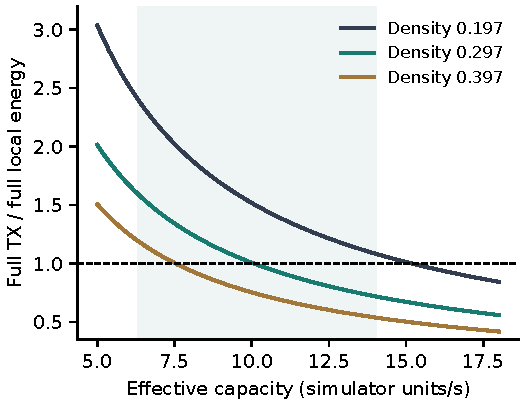
\includegraphics[width=\columnwidth]{boundary.pdf}
\caption{Full-transmission versus full-local service-energy ratio. Dashed break-even marks depend on task density and configured powers. The shaded region marks tested capacities, not calibrated RF degradation. Labels and legend are separated from the curves.}
\label{fig:boundary}\end{figure}

\section{Discussion and Limitations}
The principal result is conditional: changing effective communication service can erase a fixed policy's favorable energy--deadline tradeoff, while task-level forecasts can recover part of its service performance. Rules such as Greedy remain competitive, which tempers claims that a learned proposal is necessary for the observed correction. Forecast error, missed tasks, and per-task/full-run accounting boundaries must be examined together.

The EH contribution is a verified short-horizon trace/battery integration and training-seed ablation with modest effects. The reserve increase contains direct replenishment and changed actions; the present design does not isolate their contributions. Only a brief daytime test segment is used. Independent training across five seeds quantifies algorithm initialization variability under that shared workload/window, not uncertainty across days, deployments, or weather conditions. Longer and independently sampled trace windows, validation-based model selection, and a separately retrained non-EH policy remain needed for broad policy comparisons.

All execution is simulated. Stress weights and capacity compression are uncalibrated proxies; packet labels are not wireless measurements. The battery model neglects voltage sag, internal resistance, converter control, aging, and target-device brownout circuitry. The fixed-grid replay approximates irregular timestamps. Frozen QECO bookkeeping behavior is preserved, and EH uses a changed reward/recurrent configuration. Battery-empty service is not causally implemented in the inherited EH environment; the paper excludes post-depletion service claims. Selector/inference overhead has not been measured on hardware. The reported framework is therefore auditable and reproducible within stated assumptions, not deployment-validated.

\section{Conclusion}
Traffic-derived effective-capacity stress, paired workload replay, and explicit energy accounting reveal that device expenditure and deadline service must be reported jointly. A selector improves the frozen QECO comparison at Medium and High stress, while quantitative simple baselines prevent an unsupported claim of general superiority. Five workload seeds separately test the fixed-checkpoint comparison. Five EH training seeds support small, consistently directed short-window reserve and energy differences; their exact paired tests do not establish significance at 0.05. Combining EH-QECO with the selector exposes a useful service--energy tradeoff. Corrected task forecasts, analytical stress thresholds, and capacity-only battery-demand replay make the model's scope explicit. The resulting contribution is a reproducible simulation study of conditional offloading and EH-aware modelling, with hardware calibration and causal post-depletion service left open.

\section*{Data and Code Availability}
The public package \cite{StudyCode} contains the revised source/PDF, reviewer response, raw seed records, episode metrics, metadata audit, numerical tables, and a table-reproduction notebook. The original QECO code \cite{QECOCode}, traffic study \cite{Traffic}, and UCLM data \cite{UCLMData} are separately attributed. Raw external traffic captures are not redistributed. The package provides input hashes, download provenance, and commands for regeneration. The table-reproduction notebook reads published numerical records and rebuilds every displayed table; it does not silently retrain models. Simulation regeneration uses the documented Python/TensorFlow environment and supplied checkpoints. The frozen artifact remains identified by commit 909de4a; the revision is separately versioned.

\bibliographystyle{IEEEtran}
\bibliography{references}
\end{document}
